\chapter{Experiment}
\label{chap:experiment}
\minitoc

\section{Dataset}
\label{sec:dataset}

% \subsubsection{Synthetic Starmen dataset}

We use the \texttt{Starmen} dataset as a toy example to test and demonstrate the performance of our model. The \texttt{Starmen} dataset is a synthetic longitudinal dataset\footnote{The dataset is available at \href{https://zenodo.org/records/5081988}{https://zenodo.org/records/5081988}} consisting of $N = 1,000$ subject, each with $10$ visits at different time points. This dataset is specifically designed for studying longitudinal models, capturing both spatial and temporal variability. The temporal variability of the population is prescribed by a "starman" raising its left arm, generated according to a diffeomorphism model described in \cite{bôneStarmenDataset2018}. On the other hand, the spatial variability represents individual heterogeneity are characterized by the location of other four control points: the head, right arm and legs. This way, the effects of time progression, raising the left arm, are (spatially) independent of the inter-variability of the shapes. All subjects raise the left arm but vary in shape with different position of their legs and arms.

All images are gray scaled with 1 channel $(1 \times 64 \times 64)$, and pixel values are normalized in the range $[0, 1]$. We use $700$ patients for our training set, $150$ for validation set and $150$ for test set. We note that 1 patient has 10 visits, thus when we consider individual images we have $7000, 1500$ and $1500$ samples for train, validation and test set, respectively. We consider all images in these sets are healthy. Since this dataset does not have anomaly structure, we use \texttt{cv2} package to generate 3 types of synthetic anomaly to be used in our anomaly detection task: \texttt{growing\_circle}, \texttt{darker\_line} and \texttt{darker\_circle}. For each type of anomaly, we create an anomaly set of $20$ patients, corresponding to $200$ anomaly images. \cref{fig:example_starmen} shows 1 example of healthy patient and 3 synthetic anomaly types.

\begin{figure}
    \centering
    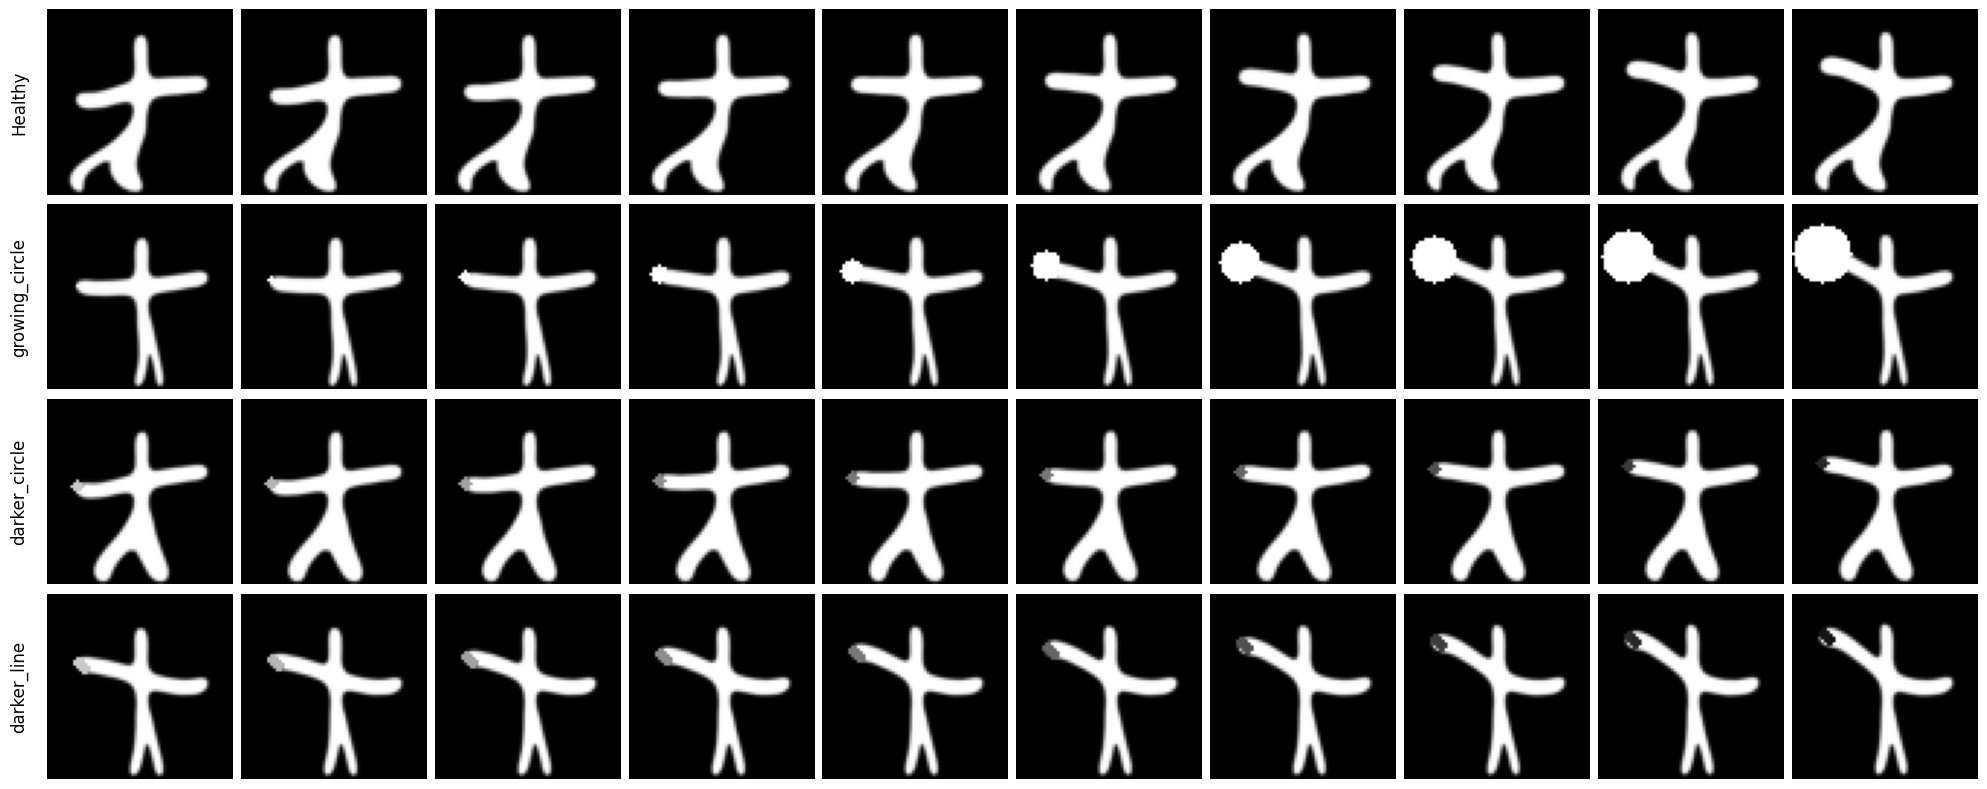
\includegraphics[width=0.75\linewidth]{figures/example_starmen.png}
    \caption[Example of \texttt{Starmen} dataset]{Examples of Starmen dataset images. The first row shows a healthy image. The last 3 rows show different anomaly type, from top to bottom: anomaly of type \texttt{growing\_circle}, anomaly of type \texttt{darker\_circle} and \texttt{darker\_line}. Each sample contains 10 sequential images at different time points, through time the mini starmen slowly raises its left hand, while maintaining all other parts of its body (head, legs and right hand). Anomalies are added using \texttt{cv2} and places at the left most points of the figure.}
    \label{fig:example_starmen}
\end{figure}

% Synthetic longitudinal dataset of starmen images  (64x64), based on the longitudinal diffeomorphic model. The cross-sectional variability of the population is prescribed by a diffeomorphism localized at four control points: the head, right arm and legs. The common progression timeline, on the other hand, is generated through a displacement of the left arm only.
% This way, the effects of time progression, raising the left arm, are (spatially) independent from the inter-variability of the shapes. All subjects raise the left arm but vary in shape with different position of their legs and arms. The dataset is comprised of $N=1000$ objects, each with $10$ visit at different time points. 

% The dynamics of progression is given by an affine reparametrization of the age at the visit, characterized by individual onset and acceleration factors, such that the true progression of the disease is given by. 

% The dataset description is given in \verb|df.csv| files, with columns: 

% \begin{itemize}
%     \item \texttt{tau}:  the onset age - the age at which a disease starts or a developmental process begins.
    
%     \item \texttt{t}: the actual age or observation time point.
    
%     \item \texttt{path}: absolute path to the subject gray scale image (1x64x64). The image is generated from `vtk` file. 
    
%     \item \texttt{id}: subject ID

%     \item \texttt{alpha}: the acceleration factor - how fast a disease developes. 
    
% \end{itemize}

% \subsubsection{Some useful github repos to process - visualize the dataset}

% \begin{itemize}
%     \item \href{https://github.com/MChen808/UOMETM/tree/main}{UOMETM repo}

% \end{itemize}

\section{Implementation details}
\label{sec:implementation}

\subsection{Spatial Diffusion Model}

\paragraph{UNet}: The baseline diffusion model is based on the DDIM model \cite{songDDIM}\footnote{Available at \href{https://github.com/openai/guideddiffusion}{https://github.com/openai/guideddiffusion}} with adaptation from LDAE \cite{lozuponeLDAE2025} \footnote{Available at \href{https://github.com/GabrieleLozupone/LDAE}{https://github.com/GabrieleLozupone/LDAE}}. The UNet comprises an input block, a middle block and an output block. The input block follows an encoder architecture that encodes and downsamples the original input. The output blocks are symmetric counterparts of the encoder, upsampling the encoded representation back to the original resolution. Each block contains one residual block (ResBlock), with channel multipliers of $[32, 64, 96]$. Each ResBlock begins with a GroupNorm layer and a SiLU activation, followed by a Conv2d layer with kernel size $(3, 3)$ and stride $(1, 1)$. Downsampling is performed with an AvgPool layer of kernel size $(2, 2)$, stride $(2, 2)$, and no padding. Attention layers are added at resolution scales of $[\tfrac{1}{2}, \tfrac{1}{4}]$ to capture dependencies across neighboring regions of the image and enhance spatial information exchange between feature maps. 
\paragraph{Condition signals}: time step condition $t$ is embedded using sinusoidal time step embeddings, originated from \cite{vaswani2023attentionneed}. The embedded $t$ is then projected through a linear layer followed by a SiLU activation to obtain a vector of dimension $d_{cond} = 128$. We use ResNet50 as the backbone for the semantic encoder $\mathrm{Enc}{\phi}$. The parameters $\phi$ are initialized from the pretrained ResNet module in PyTorch. The final classifier layer of ResNet is replaced with a fully connected layer to produce a non-spatial representation of the input, $\rvy_{sem} = \mathrm{Enc}_{\phi}(\rvx)$, with latent dimension $d = 512$. This representation is further projected via linear layers to match the dimension of the time step embedding. Finally, the conditioning variables $(\rvy_{sem}, t)$ are injected into the network using AdaGN. 
\paragraph{Training configuration}: \ac{SDM} is trained with a total number of diffusion time steps $T = 1000$ and a linear noise variance from $\beta_1 = 0.0001$ to $\beta_T = 0.02$. We use the Adam optimizer with a learning rate of $2 \times 10^{-5}$. Training is performed for 500 epochs with a training batch size of $2$ patients, corresponding to an effective batch size of $20$ samples. Following common practice in diffusion models \cite{lozuponeLDAE2025, rombachLDM}, we use an exponential moving average (EMA) to stabilize training and improve generalization. EMA decay rate is $0.999$, and EMA parameters are updated after every 10 batches. A full list of architectural and training parameters is provided in \cref{tab:sdm-config}.

\begin{table}[h]
\captionsetup{justification=raggedright,singlelinecheck=false}
\caption{Spatial Diffusion Model (SDM): configurations and parameters}
% \resizebox{\columnwidth}{!}{%

\begin{adjustbox}{max width=0.9\textwidth}
    \begin{tabular}{ll}
    \toprule
    \multicolumn{2}{l}{\textbf{Semantic Encoder $\mathrm{Enc}_{\phi}$}} \\
    \midrule
    Backbone & \texttt{ResNet50}\cite{ResNet50} \\
    Pretrained Init & ImageNet \\
    Input Modality & $1 \times 64 \times 64 $ \\
    Output layer & \texttt{Linear(in=1000, out=512)} \\
    Output Representation & non-spatial vector $\mathbf{y}_{sem} \in \mathbb{R}^{512}$ \\
    \midrule
    \multicolumn{2}{l}{\textbf{Diffusion UNet $\epsilon_{\theta}$}} \\
    \midrule
    Input Shape & $(B, 1, 64, 64)$, with batch size first \\
    Channels multipliers & [32, 64, 96] \\
    Residual Blocks per Level & 1 \\
    Attention Resolutions (factors) & [2, 4] \\
    Number of attention head & 1 \\
    Conditional injection & AdaGN (scale-shift norm) \\
    Dropout & 0.1 \\
    Time embedded dimension & $d_{cond} = 128$ \\
    Semantic encoder dimension & $d_{sem}=512$ \\
    Timestep & 1000 \\
    Beta Schedule & Linear, $\beta_t \in [10^{-4}, 2 \times 10^{-2}]$ \\
    \midrule
    \multicolumn{2}{l}{\textbf{Training Configuration}} \\
    \midrule
    Optimizer & Adam \\
    Learning Rate & $2.5 \times 10^{-5}$ \\
    EMA Decay & 0.999 \\
    Train Batch Size (effective) & 20 \\
    Training Duration & 500 epochs / $\sim$3 hours \\
    Hardware & 2 x Nvidia L40S (45 GiB) \\
    \bottomrule
    \end{tabular}
\end{adjustbox}
% }
\label{tab:sdm-config}
\end{table}

\subsection{Feature Extractor network of FAM}

Our FE network $\Phi$ is initialized from trained semantic encoder $\mathrm{Enc}_{\phi}$. To learn the similarity between samples, each training batch $\rvx \in \mathbb{R}^{B \times 1 \times 64 \times 64}$ is passed through the SDM model to obtain its reconstruction $\widehat{\rvx} \in \mathbb{R}^{B \times 1 \times 64 \times 64}$. We employ the DDIM sampling scheme in the denoising process with 100 steps to accelerate training. To improve generalization, we reconstruct $\rvx$ from different noise levels $[100, 250, 500, 1000]$, selected uniformly at each epoch. Cosine similarity loss is calculated on three layers of ResNet50, each at a different resolution, and the losses are summed to obtain the total loss. Distillation loss is incorporated from frozen $\mathrm{Enc}_{\phi}$ network, with parameter $\lambda_{DL} = 1$, using \cref{eq:fe-dl-loss}. FE is trained with 100 epochs, using Adam optimizer with learning rate $10^{-4}$. \cref{tab:fe-config} shows the details configurations of our FE network.  

\begin{table}[h]
\captionsetup{justification=raggedright,singlelinecheck=false}
\caption{Feature Extractor network (FE): configurations and parameters}
% \resizebox{\columnwidth}{!}{%
\begin{tabular}{ll}
\toprule
\multicolumn{2}{l}{\textbf{FE $\Phi$}} \\
\midrule
Backbone & \texttt{ResNet50}\cite{ResNet50} \\
Pretrained Init & Semantic Encoder $\mathrm{Enc}_{\phi}$ \\
Architecture & Same as $\mathrm{Enc}_{\phi}$ \\
Input Shape & $(B, 1, 64, 64)$, with leading dimension is batch size \\
Feature layers & [\texttt{layer1, layer2, layer3}] \\
Feature size - \texttt{layer1} & [256, 64, 64] \\
Feature size - \texttt{layer2} & [512, 8, 8] \\
Feature size - \texttt{layer3} & [1024, 4, 4] \\
DDIM samle step & 100 \\
Noise level & [100, 250, 500, 1000] \\
$\lambda_{DL}$ & 0.1 \\
Optimizer & Adam \\
Learning Rate & $1.0 \times 10^{-4}$ \\
Train Batch Size (effective) & 20 \\
Training Duration & 100 epochs / $\sim$4 hours \\
Hardware & 1 x Nvidia L40S (45 GiB) \\
\bottomrule
\end{tabular}
% }
\label{tab:fe-config}
\end{table}

\section{Evaluation metrics}

The performance of our model is evaluated based on two main criteria: reconstruction quality and anomaly detection score. In this section, we outline the details of our evaluation metrics for both tasks. 

\subsection{Reconstruction quality}

For both SDM and TDM, the goal of diffusion model is to reconstruct the ground truth image: it can be the original healthy image (in the case of SDM), or the ground truth missing image (in the case of TDM). To evaluate the overall reconstruction quality, we follow conventional methods in literature \cite{rombachLDM, lozuponeLDAE2025, behrendt2025cDDPM}, and calculate both pixel error metrics and similarity metrics between inputs and reconstructed images. For pixel error, we report both the $l1$ and $l2$ errors. For similarity, we consider the Structural Similarity Index Measure (SSIM), the Peak Signal To Noise Ratio (PSNR) and the Learned Perceptual Image Patch Similarity (LPIPS) as metrics to assess the reconstruction quality. To account for perceptual structures at both coarse scales and fine details scales, we also calculate the Multi Scale Structural Similarity (MSSIM), which is more aligned with human visual perception. For the feature based LPIPs metric, features are extracted by a \texttt{squeeze} network. All similarity metrics are implemented in \texttt{Monai} package \footnote{MONAI is an open-source framework for deep learning in healthcare imaging, available at \href{https://docs.monai.io/en/stable/index.html}{https://docs.monai.io/en/stable/index.html}}. 

Furthermore, for anomaly detection task, only healthy anatomy should be reconstructed. Similar to \cite{behrendt2025cDDPM}, we consider the $l1$-error of healthy and unhealthy anatomy separately, given the synthetic anomaly data sets. Specifically, we calculate the $l1$-error for both healthy and unhealthy anatomy, as indicated by the annotation masks and also calculate an $l1$-ratio as follows:
\begin{equation}
    l1\text{-ratio} = \frac{l1_{anomaly}}{l1_{healthy}}
    \label{eq:l1-ratio}
\end{equation}

For healthy region, we want to have as small error as possible, while for anomaly region it is better to have higher errors, which will help to separate anomaly part from healthy structure. A higher value for $l1$-ratio indicates that the model successfully remove the anomaly region while maintaining correct structure of healthy anatomy, and vice versa. 

\subsection{Anomaly scores}

To evaluate the performance of our models in anomaly detection, we use the ground-truth segmentation from our synthetic anomaly dataset. It is important to note that ground-truth labels/annotations are often unavailable in real-life MRI datasets, especially in unsupervised settings. Nevertheless, most common models still rely on datasets with ground-truth labels to assess their performance, as reported in Bercea’s study \cite{berceaDDPMforMedicalImagesStudy2024}.

\textbf{Image-level anomaly detection}: recall from \cref{sec:post-process} that from a spatial anomaly score map, we use several functions to summarize all pixel-level score into 1 single value that we can assign for image level anomaly score. The AUROC and AUPRC are popular metrics \cite{wu2024maskdiffusionposteriorMDPS, behrendt2025cDDPM, DDAD, wangEPDiffErasurePerception2025} due to their threshold independence, so we can assess the model's performance directly from raw anomaly score without having to find a threshold value. However, AUROC is reported to have potential misleading in imbalanced datasets dominated by the majority class \cite{berceaDDPMforMedicalImagesStudy2024}. The AUPRC focuses on precision recall trade-offs and offers better evaluations in imbalanced datasets where anomalies are scarce. 

\textbf{Pixel-level anomaly localization}: at pixel level, we care about the segmentation of anomaly. Following \cite{behrendt2025cDDPM, wangEPDiffErasurePerception2025}, we use the Dice score metric, which measures the overlap between the predicted and ground truth segmentations, providing a single value that balances false positives and false negatives \cite{berceaDDPMforMedicalImagesStudy2024}. The Dice score is given by: 

\begin{equation}
    \label{eq:dice-score}
    \mathrm{DICE} = \frac{2. |A \cap B|}{|A| + |B|}
\end{equation}

where $A$ and $B$ are the anomaly map and the ground truth segmentation, respectively. One disadvantage of this metric is that it requires setting a threshold value from our anomaly score maps to determine whether a pixel is classified as anomalous, which can significantly impact results. As mentioned in \cref{sec:post-process}, we will use Yen threshold technique, which can provide automatic threshold value without using any greedy search algorithm.  